\documentclass[11pt,a4paper]{article}
\usepackage[top=40px, left=60px, right=60px]{geometry}
\usepackage[T1]{fontenc}
\usepackage[normalem]{ulem}
\usepackage{verbatim}
\usepackage[utf8]{inputenc}
\usepackage[francais]{babel}
\usepackage{graphicx}
\usepackage{placeins}
\usepackage{listings}
\usepackage{setspace}
\usepackage{color}
\usepackage{amsmath}
\usepackage{amsfonts}
\usepackage{amssymb}
\usepackage{url}

\definecolor{mygreen}{rgb}{0,0.6,0}
\definecolor{mygray}{rgb}{0.5,0.5,0.5}
\definecolor{mymauve}{rgb}{0.58,0,0.82}

\lstset{ %
  basicstyle=\footnotesize\ttfamily,
  frame=single,
  backgroundcolor=\color{white},   % choose the background color
  basicstyle=\footnotesize,        % size of fonts used for the code
  breaklines=true,                 % automatic line breaking only at whitespace
  captionpos=b,                    % sets the caption-position to bottom
  commentstyle=\color{mygreen},    % comment style
  escapeinside={\%*}{*)},          % if you want to add LaTeX within your code
  keywordstyle=\color{blue},       % keyword style
  stringstyle=\color{mymauve},     % string literal style
  numbers=left,
  literate=
  {á}{{\'a}}1 {é}{{\'e}}1 {í}{{\'i}}1 {ó}{{\'o}}1 {ú}{{\'u}}1
  {Á}{{\'A}}1 {É}{{\'E}}1 {Í}{{\'I}}1 {Ó}{{\'O}}1 {Ú}{{\'U}}1
  {à}{{\`a}}1 {è}{{\'e}}1 {ì}{{\`i}}1 {ò}{{\`o}}1 {ù}{{\`u}}1
  {À}{{\`A}}1 {È}{{\'E}}1 {Ì}{{\`I}}1 {Ò}{{\`O}}1 {Ù}{{\`U}}1
  {ä}{{\"a}}1 {ë}{{\"e}}1 {ï}{{\"i}}1 {ö}{{\"o}}1 {ü}{{\"u}}1
  {Ä}{{\"A}}1 {Ë}{{\"E}}1 {Ï}{{\"I}}1 {Ö}{{\"O}}1 {Ü}{{\"U}}1
  {â}{{\^a}}1 {ê}{{\^e}}1 {î}{{\^i}}1 {ô}{{\^o}}1 {û}{{\^u}}1
  {Â}{{\^A}}1 {Ê}{{\^E}}1 {Î}{{\^I}}1 {Ô}{{\^O}}1 {Û}{{\^U}}1
  {œ}{{\oe}}1 {Œ}{{\OE}}1 {æ}{{\ae}}1 {Æ}{{\AE}}1 {ß}{{\ss}}1
  {ç}{{\c c}}1 {Ç}{{\c C}}1 {ø}{{\o}}1 {å}{{\r a}}1 {Å}{{\r A}}1
  {€}{{\EUR}}1 {£}{{\pounds}}1
}

\title{Factorisation d'entiers}
\author{Stéphane Horte \& Gabriel Lewertowski}

\begin{document}
\maketitle

\tableofcontents
\newpage

\begin{abstract}
Nous présentons trois algorithmes de factorisation d'entiers : les algorithmes \textit{$\rho$} et \textit{$(p-1)$} proposés par J.M Pollard en 1974 dans \cite{pollard_rho} ainsi que l'algorithme \textit{ECM} (Elliptic Curve Method) décrit par H. W. Lenstra, Jr dans \cite{lenstra}. Nous testons ensuite nos implémentations sur des grands nombres choisis aléatoirement, et nous comparons avec les résultats obtenus par \textsf{GMP-ECM}.
\end{abstract}

\section{Présentation des algorithmes}
\subsection{Algorithme $\rho$ de Pollard}
Introduit en 1975 par John M. Pollard \cite{pollard_rho}, l'algorithme $\rho$ (parfois Monte-Carlo) est très efficace pour déterminer des petits facteurs premiers (de l'ordre de 10 chiffres). Des améliorations furent proposées, notamment en 1985 par Brent \cite{brent85} pour réduire le nombre de calculs effectués. Nous nous intéressons ici à la version initiale de John M. Pollard, qui trouve un facteur premier $p$ en $O(\sqrt{p})$ itérations.
\subsubsection{Principe de fonctionnement}
\label{rho}

Soit $N$ un entier quelconque à factoriser.
	
Nous nous plaçons dans $\mathbb{Z}/N\mathbb{Z}$. Soit $f$ une fonction polynomiale d'ordre au moins 2 et à coefficients dans  $\mathbb{Z}$. Par compatibilité de l'addition et de la multiplication avec la réduction modulo $N$, $f$ définit une fonction de $\mathbb{Z}/N\mathbb{Z}$ dans $\mathbb{Z}/N\mathbb{Z}$. Pour toutes fonctions polynomiales réduites modulo $N$ et pour tout $x_0$ élément de $\mathbb{Z}/N\mathbb{Z}$, on définit la suite des itérations  $(x_i)_{i \in \mathbb{N}}$ avec $x_i$ = $f^i(x_0)$. La suite des $(x_i)_{i \in \mathbb{N}}$ est à valeurs dans un ensemble fini. Par conséquent il existe forcément deux indices $i \neq j$ tels que $x_i$ = $x_j$. Soit ($i,j$) le plus petit couple (pour l'ordre lexicographique) qui vérifie cette propriété. La période de la suite est donc $j-i = \lambda$. On remarque aussi que pour tout $k$ et $l$ dans $\mathbb{N}$ on a $x_{i+k}$ = $x_{j+k+l\lambda}$. Par conséquent on peut trouver un entier $t$ tels que $x_t$ = $x_{2t}$. Le plus petit $e$ vérifiant cette propriété s'appelle \textbf{l'épacte} et est noté $e$. Il est démontré les résultats suivants :
	
\begin{equation}
	\mathbb{E}(\lambda) = \sqrt { \frac{N\pi}{8} } + O(1) \approx 0.627 \sqrt N + O(1) \nonumber
\end{equation}	
\begin{equation}
	\mathbb{E}(e) = \sqrt { \frac{N\pi^5}{288} } + O(1) \approx 1.03 \sqrt N + O(1) \nonumber
\end{equation}	
où $\mathbb{E}$ désigne l'espérance probabiliste. \\

Soit $p$ un facteur de $N$ encore inconnu. La fonction $f$ se réduit à une fonction de $\mathbb{Z}/p\mathbb{Z}$ dans $\mathbb{Z}/p\mathbb{Z}$ en prenant sa réduction modulo $p$ de sa réduction modulo $N$. Par les théorèmes énoncés précédemment nous sommes capables de trouver en un nombre d'étapes $O(\sqrt p)$ un entier $l$ tel que $x_l$ = $x_{2l}$ modulo $p$. Pour un tel indice, $p$ divise $x_l-x_{2l}$ et par conséquent $p$ divise aussi le pgcd de $N$ et de $x_l-x_{2l}$. C'est dans ce résultat que réside le principe de la méthode $\rho$ de Pollard : Pour chercher un facteur de $N$ il nous suffit alors de calculer les pgcd successifs de $N$ et de $x_i-x_{2i}$ pour $i=1, 2, \ldots$.
	
L'avantage de cet algorithme par rapport à un test trivial de divisibilité par tous les nombres inférieurs à $\sqrt{N}$ est immédiat : on obtient une complexité $O(\sqrt{p})$ au lieu de $O(\sqrt{N})$. Remarquons que nous n'avons pas besoin de connaître explicitement $p$ pour appliquer la méthode $\rho$.

\subsubsection{Notre code}
Pour chacun des algorithmes $\rho$, $p-1$ et \textit{ECM}, nous implémentons en python une fonction \textit{un\_facteur} qui trouve un facteur premier. Cette fonction peut avoir recours au test de primalité de Miller-Rabbin, dont l'implémentation est donnée en Annexe. Enfin, pour chaque algorithme, une fonction \textit{factorise} (voir également le code en Annexe) permet de factoriser totalement un entier. 

\lstinputlisting[language=Python, firstline=1, lastline=29]{../pollard.py}

\subsection{La méthode $p-1$}
La méthode $\rho$ que nous venons d'étudier ne présuppose aucune hypothèse sur l'entier $N$ à factoriser. Dans le cas où $N$ possède un facteur premier $p$ tel que $p-1$ est \textbf{friable}, c'est-à-dire qu'il ne possède que des petits facteurs premiers, la méthode $p-1$, également inventée par John M. Pollard, permet de trouver $p$ plus rapidement.

\subsubsection{Le principe de fonctionnement}

Le principe de l'algorithme $p-1$ repose sur le théorème de Fermat : si $p$ est un nombre premier et si $a$ est un entier non divisible par $p$ alors $a^{p-1} \equiv 0 \pmod p$.
	
	 Considérons encore une fois $N$ le nombre que nous cherchons à décomposer et $p$ un de ses facteurs à priori inconnu. Soit $a \in \{2,\ldots,N-2\}$ premier avec $N$. \\

\textbf{La première phase}

Soit $B_1$ une borne, typiquement $B_1 = 10^6$. Soit $R = ppcm (1,2,...,B_1)$. On calcule ensuite le nombre $b \equiv a^{R} \pmod N$ en un temps $O(B_1)$. Si $p-1$ divise $R$ alors, par le théorème de Fermat on a $p$ qui divise $b-1$, et donc le pgcd de $b-1$ et de $N$. $pgcd(b-1, N)$ est donc un facteur de $N$, non nécessairement premier puisque tous les facteurs $q$ de $N$ tels que $q-1$ divise $R$ apparaissent dans $pgcd(b-1, N)$. La première étape a échoué si $d=pgcd(p,a^{R-1})$ vaut 1 ou $N$. Si $d = 1$ alors deux solutions existent : 
\begin{itemize}
\item recommencer avec une borne $B_1$ plus grande
\item passer à l'étape 2 (voir plus loin)
\end{itemize}
\medskip 
Remarque : si $d = N$, tous les facteurs $q$ de $N$ sont tels que $q-1$ divise $R$, il faut donc recommencer avec $B_1$ plus petit. \\
	 
Cette étape nécessite que tous les facteurs de $p-1$ soient petits. Cette technique n'est donc clairement pas efficace si $p-1$ est, par exemple, la multiplication de deux nombres premiers de tailles équivalentes. On peut cependant remarquer que la première étape finira toujours par renvoyer un facteur $p$ de $N$ quitte à augmenter $B_1$. \\

\textbf{La seconde phase}

La seconde phase requiert une autre borne $B_2 \gg B_1$, par exemple $B_2 = 1000B_1$. On suppose que $p-1$ n'a qu'un seul grand facteur premier dans sa décomposition, c'est à dire $p-1 = sh $ avec $h$ qui divise $R$ de la première phase et $B_1 \leqslant s \leqslant B_1$. Pour tous les $s$ nombre premier entre $B_1$ et $B_2$ on calcule $T_s$ = $b^s$ = $a^{Rs}$. On calcule ensuite $d_s = pgcd(N,T_s)$ en espérant que celui ci soit différent de 1. Comme expliqué dans la première phase, si $p-1$ divise $R \cdot s$ alors $p$ divise $T_s$ et $p$ divise $d_s$. Comme dans la première phase on remarque que dans le cas où $d_s > 1$ alors $d_s$ est un facteur de $N$ mais pas obligatoirement un facteur premier. La seconde phase à une complexité de l'ordre de $\log(B_2)^2$. Encore une fois, dans le cas où $p-1$ possède au moins deux grands nombres premiers dans sa décomposition, la méthode $p-1$, même accompagnée de la seconde phase, n'est pas très efficace. \\
	
\textbf{Commentaires}
	
	Cette méthode repose, tout comme le théorème de Fermat, sur l'ordre du groupe multiplicatif $(\mathbb{Z}/p\mathbb{Z})^*$ qui vaut $p-1$ et sur le théorème de Lagrange qui stipule que l'ordre d'un élément divise forcément l'ordre du groupe. L'idée de se déplacer dans un groupe associé à $p$ est très intéressante. Les méthodes $p+1$ et \textit{ECM} (Elliptic Curve Method) sont très largement inspirées de cette technique en se plaçant sur d'autres groupes, faisant ainsi d'autres hypothèses sur l'écriture des facteurs de $N$. 

\subsubsection{Notre code}

\lstinputlisting[language=Python, firstline=1, lastline=53]{../pmoinsun.py}

\subsection{La méthode \textit{ECM}}

	La méthode \textit{ECM} propose le même raisonnement que $p-1$ mais en se plaçant sur les courbes elliptiques sur $\mathbb{Z}/N\mathbb{Z}$. Pour $N$ non premier, les points d'une courbe elliptique sur $\mathbb{Z}/N\mathbb{Z}$ ne forment pas un groupe car l'addition de deux points de la courbe nécessite l'inversion d'un facteur, qui peut être non inversible dans $\mathbb{Z}/N\mathbb{Z}$. Cependant, si ce facteur est non inversible, c'est qu'il n'est pas premier avec $N$ : un facteur de $N$ est dès lors trouvé. 
	
\subsubsection{Les courbes elliptiques}
	
	Nous prendrons couramment l'écriture de Weierstrass pour définir les courbes elliptiques. Une courbe elliptique dans $\mathbb{Z}/N\mathbb{Z}$ est définie par la donnée de deux coefficients $A$ et $B$ tels que $4A^3+27B^2 \ne 0$. Ce sont les points $(X,Y)$ de $(\mathbb{Z}/N\mathbb{Z})^2$ qui vérifient
\begin{equation}
	Y^2 = X^3 + A X +b
\end{equation}

	Il est évident, pour les raisons exposées en \ref{rho}, qu'une courbe elliptique dans $\mathbb{Z}/N\mathbb{Z}$ définit aussi une courbe elliptique dans $\mathbb{Z}/p\mathbb{Z}$. Cette courbe elliptique définit bien un groupe car $p$ est premier. Ce groupe est d'ordre $p+1-t_{A,B}$ où $t_{A,B}$ dépend de $A$ et $B$ avec $|t_{A,B}| \leqslant 2 \sqrt{p}$ (théorème de Hasse). Tout comme l'algorithme $p-1$ réussit si $p-1$ est \textbf{friable}, la méthode \textit{ECM} réussit si $p+1-t_{A,B}$ est friable. La grande force de la méthode \textit{ECM} est qu'il est peu probable que deux courbes elliptiques aient le même ordre. En effectuant l'algorithme avec une courbe choisie aléatoirement, l'ordre du groupe varie à chaque itération, ce qui multiplie la probabilité de succès par rapport à $p-1$. 

Dans ce cas il est même possible de calculer  le point  $k \cdot(x,y)$  en un temps  $O(\log_2(k))$. Si un point est écrit grâce à la forme homogénéisé $(x,y,z)$ alors c'est le $0$ de la courbe modulo $p$ si et seulement si $p$ divise $z$. C'est ce que nous serons amenés à tester.

À nouveau, l'algorithme se présente comme une succession de deux phases. \\
	
\textbf{La première phase}
\label{mult_rapide}

La première phase est équivalente à la première phase de la méthode $p-1$. Soit $B_1$ une borne. Nous choisissons (à priori aléatoirement) une courbe elliptique et un point sur cette courbe. Dans la pratique, il est plus facile de choisir un point $P_0 =(x_0,y_0,1)$ et un coefficient $A$ puis chercher  $B$ tel que la courbe définie grâce à $A$ et $B$ passe par le point $P_0$. Nous posons de manière analogue $R = ppcm (1,2,..,B_1)$ puis nous calculons le point $R \cdot P_0 $ en un nombre d'opérations de l'ordre de $\log(R)= O(B_1)$. Pour cela, l'utilisation de l'équation homogène
\[
Z Y^2 = X^3 + A Z ^2 X + Z^3 b
\]
permet une multiplication rapide en évitant le calcul d'inverses.

Si l'ordre du groupe des points de la courbe elliptique divise $R$, alors le point $R \cdot P_0 = (x,y,z)$ est égal à $O_E$, l'élément neutre de la courbe (i.e $p | z$). Le test de fin de la première phase est donc le calcul de $d = pgcd (N,z)$, qui fournit un diviseur de $N$ lorsque $1 < d < N$. On dit que la première phase a échoué si $d = 1$ ou $d=N $. Si $d = N$, on peut recommencer avec cette courbe elliptique et une borne $B_1$ plus petite ou recommencer avec une autre courbe. Si $d=1$ on peut recommencer avec une borne $B_1$ plus grande, passer à la seconde phase ou changer de courbe et reprendre à la phase 1. \\

\textbf{La seconde phase}
	
Pour la seconde phase nous nous donnons une borne $B_2 \gg B_1$. Nous repartons du point $Q = R \cdot P_0$ calculé durant la phase précédente. Pour tous les nombres premiers $s$ compris entre $B_1$ et $B_2$ nous remplaçons $Q$ par $ s \cdot Q$. Une fois tous les nombres premiers compris entre $B_1$ et $B_2$ passés il ne reste qu'à calculer $d = pgcd(z,N)$ ou $z$ représente la troisième coordonnée de $Q$. À nouveau, si $1 < d < N$, on a trouvé un diviseur de N. Si $d = 1$ il faut augmenter les bornes ou bien recommencer avec une autre courbe de façon à changer le cardinal du groupe sur lequel nous travaillons. Si $d = N$, on peut à souhait recommencer sur une autre courbe ou baisser la borne $B_2$ sur la même courbe. La seconde phase est une version allégée de la première phase. En effet, cela revient à supposer qu'il n'est plus nécessaire de prendre en compte les puissances de "petits" nombres premiers trop grandes. Par exemple, la plus grande puissance de $2$ considérée est $2^{[\log(B_1)]}$. Contrairement à la méthode $p-1$, le pire cas n'est pas celui où le cardinal du groupe s'écrit comme produit de deux "grands" nombres premiers mais le cas où un "grand" nombre premier apparaît à une puissance au moins 2 dans la décomposition de l'ordre du groupe. 

\subsubsection{Notre code}
\lstinputlisting[language=Python, firstline=1, lastline=76]{../ECM.py}

\section{\textit{ECM}, hier et aujourd'hui}
La méthode \textit{ECM} a été proposée par H. W. Lenstra en 1985 \cite{lenstra}, et peu d'améliorations ont été apportées depuis. Alors qu'à ses débuts, l'algorithme permet de trouver des facteurs premiers de 30 chiffres au maximum, R. Brent prédit qu'\textit{ECM} permettra à l'avenir de trouver des facteurs premiers de 50 chiffres. En effet, dix ans plus tard en 1995, P. Montgomery trouve un facteur de 47 chiffres de $5^{256} +1$. L'actuel record est un facteur de 83 chiffres, trouvé en septembre 2013 par R. Propper en factorisant $7^{337}+1$ \cite{records_ecm}. \\

P. Montgomery et R. Propper se sont intéressés à ces nombres dans le cadre du Projet Cunningham, lancé en 1925 et visant à factoriser des entiers de la forme $b^n \pm 1$ avec $b \in \{2, 3, 5, 6, 7, 10, 11, 12\}$ et $n$ grand. \textit{ECM} fait partie, avec le crible algébrique et le crible quadratique à polynômes multiples, des trois seuls algorithmes utilisés actuellement pour factoriser ces nombres. \\

Aujourd'hui, l'algorithme \textit{ECM} est le meilleur algorithme de factorisation connu parmi ceux pour lesquels la complexité dépend de la taille du facteur trouvé et non de la taille de l'entier à factoriser : on ne considère donc pas le crible quadratique et le crible algébrique, dont les complexités respectives en fonction de l'entier $n$ à factoriser valent $O\left(e^{\sqrt{\log n\log\log n}}\right)$ et $O\left(e^{(\frac{64}{9}\log n)^{\frac{1}{3}}(\log\log n)^{\frac{2}{3}}}\right)$. \\

L'implémentation la plus rapide de l'algorithme \textit{ECM} est \textsf{GMP-ECM}, un programme développé en C par des chercheurs de l'INRIA, permettant de factoriser un entier avec les méthodes $p-1$, $p+1$ et \textit{ECM}.

\subsection{Fonctionnement de \textsf{GMP-ECM}}
Le programme prend en paramètre la borne $B_1$ de l'étape 1 et un ou plusieurs entiers à factoriser depuis   l'entrée standard. Par exemple, pour factoriser un entier avec $B_1 = 10^6$ :


\begin{figure}[!h]
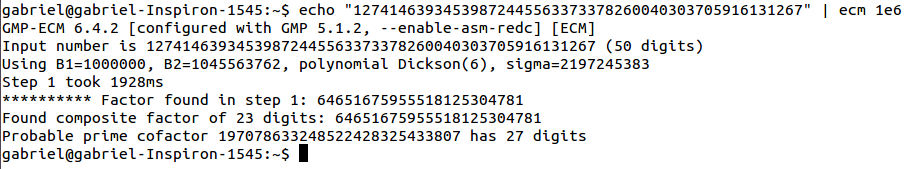
\includegraphics[scale=0.5]{images/gmp-ecm1.png}
\end{figure}

Par défaut, la méthode utilisée est \textit{ECM}. On peut utiliser $p-1$ avec l'option -pm1 : 

\begin{lstlisting}[language=bash]
	echo "12652209139612535291" | ecm -pm1 1e6
\end{lstlisting}

L'utilisateur peut également spécifier une valeur de $B_2$ pour la phase 2. Par exemple, pour utiliser $B_1=10^6$ et $B_2=10^9$ : 

\begin{lstlisting}[language=bash]
	echo "12652209139612535291" | ecm 1e6 1e9
\end{lstlisting}

Si aucune valeur de $B_2$ n'est spécifiée, \textsf{GMP-ECM} détermine automatiquement la valeur de $B_2$ optimale en fonction de la taille de l'entier à factoriser.
\medskip

\begin{tabular}{|c|c|c|c|}
  \hline
  Nb de chiffres de $N$ & $B_1$ optimal & $B_2$ optimal & Nb de courbes à utiliser \\
  \hline
  20 & 11e3 & 1.9e6 	& 74  \\
  25 & 5e4 & 1.3e7 & 214 \\
  30 & 25e4 & 1.3e8 & 430 \\
  35 & 1e6 & 1.0e9 & 904 \\
  40 & 3e6 & 5.7e9 & 2350 \\
  45 & 11e6 & 3.5e10 & 4480 \\
  50 & 43e6 & 2.4e11 & 7553 \\
  55 & 11e7 & 7.8e11 & 17769 \\
  60 & 26e7 & 3.2e12 & 42017 \\
  65 & 85e7 & 1.6e13 & 69408 \\
  \hline
\end{tabular}

\subsection{Détails de l'implémentation}
L'algorithme \textit{ECM} tel que présenté en 1985 par Lenstra sélectionnait aléatoirement la courbe elliptique sur laquelle travailler. P. Montgomery a proposé en 1987 dans \cite{montgomery} une amélioration pour travailler avec une famille infinie de courbes dont l'ordre est divisible par 12, ce qui augmente la probabilité de succès puisque l'algorithme \textit{ECM} réussit si l'ordre du groupe n'a que des petits facteurs. C'est cette famille de courbes qu'utilise \textsf{GMP-ECM}, avec la paramétrisation 
\[
by^2z = x^3 + ax^2z + xz^2
\]
qui permet une addition et une multiplication rapides comme nous l'avons vu en \ref{mult_rapide}. \\

Lors de la phase 2, \textsf{GMP-ECM} a recours à l'extension de Brent-Suyama qui, au lieu de calculer $b^s$ pour $s$ un nombre premier dans l'intervalle $[B_1, B_2]$, calcule $b^{(6k)^e - 1}$ avec $k$ un entier et $e$ un petit entier pair. Cette extension utilise la remarque suivante : tout nombre premier strictement supérieur à 3 est de la forme $6k \pm 1$. Pour plus de détails sur l'extension de Brent-Suyama et l'évaluation multipoints, voir \cite{zimmerman}.

\section{Résultats expérimentaux}

\subsection{Protocole}
Pour tester les différents algorithmes de factorisation, nous avons cherché à factoriser des entiers "aléatoires" comportant $10, 20, \ldots, 200$ chiffres. Pour cela, nous avons utilisé les décimales de $\pi$ : 

\lstinputlisting[language=Python, firstline=195, lastline=203]{../utils.py}

où \textit{pi.txt} est un fichier contenant les 500 premières décimales de $\pi$. Nous avons ainsi effectué 100 tests différents pour chaque taille d'entiers et pour les algorithmes suivants :
\begin{itemize}
\item \textit{$p-1$} sans phase 2
\item \textit{$p-1$} avec phase 2
\item \textit{ECM} testé sur 5 courbes
\item \textit{ECM} testé sur 50 courbes
\end{itemize}
\medskip
Le test est réussi si l'entier a été entièrement factorisé. Ici, seule nous intéresse la faisabilité et non la rapidité : nous avons donc utilisé \textsf{GMP-ECM} plutôt que nos implémentations. 

\subsection{Résultats pour $B_1=10^4$}




\section{Annexe}
Nous détaillons ici l'implémentation des fonctions arithmétiques utilisées.

\subsection{AMR}
\lstinputlisting[language=Python, firstline=12, lastline=53]{../utils.py}

\subsection{Crible d'Eratosthène segmenté}
\lstinputlisting[language=Python, firstline=75, lastline=100]{../utils.py}


\begin{thebibliography}{9}
\bibitem{pollard_rho}
J. M. Pollard, \emph{A Monte Carlo method for factorization}, BIT, 1975, pp.331-334

\bibitem{monte_carlo}
J. M. Pollard, \emph{Monte Carlo methods for index computation (mod p)}, Mathematics of computation, Vol. 32, No.143 (Juillet 1978), pp. 918-924

\bibitem{brent85}
R. P. Brent, \emph{An improved Monte Carlo factorization algorithm}, BIT, 1980, pp.176-184

\bibitem{lenstra}
H. W. Lenstra, Jr, \emph{Factoring integers with elliptic curves}, Annals of Mathematics, 1987, pp.649-673

\bibitem{montgomery}
P. Montgomery, \emph{Speeding the Pollard and Elliptic curve methods of factorization}, American Mathematical Society, jan. 1987, pp. 243-264

\bibitem{zimmerman}
P. Zimmerman, \emph{\textsf{GMP-ECM}: yet another implementation of the Elliptic Curve Method}, conférence.

\bibitem{zimmermandodson}
Paul Zimmermann \& Bruce Dodson, \emph{20 years of ECM}

\bibitem{records_ecm}
\url{http://www.loria.fr/~zimmerma/records/top50.html}

\bibitem{ecm_readme}
ECM README, \url{http://srawlins.ruhoh.com/ecm_readme/}

\end{thebibliography}

\end{document}
